{\chapter{Background}}
\label{sec:background}

\section{Organic Semiconductors}

%When atoms bond together, molecular orbital are defined by the linear combination of atomic orbitals, however the symmetry shown on some complex structures are not explained by a simple linear combination, instead hybrid atomic orbitals are formed. This mathematical process is called \textbf{hybridization}.
Unlike inorganic semiconductors, organic semiconductors are lightweight, easy to chemical tune, mechanical flexible, and possess low-cost and low-temperature processing. All of these characteristics increased the attention to this type of materials in the field of organic electronics. 

%\subsection{Conjugated polymers}
%\subsection{Small molecules}

\subsection{Electronic Structure}

Organic semiconductors are $\pi$-conjugated molecules that comprise mostly carbon and hydrogen atoms, with alternating multiple (sp$^{3}$, sp$^{2}$ hybridization) and single (sp hybrization) bonds. This configuration exhibit $p$ orbitals with delocalized electrons, charge transport among the length of these polymers is caused by this resonance structure. 
Based on the size of the conjugated system, organic semiconductors can be divided into conjugated polymers and small molecules.

\subsubsection{Conjugated polymers}
%Semiconducting properties of conjugated polymers built by alternating electron donor and acceptor moieties \cite{mattElectronicStructureMorphology2021}, 
%Since inorganic semiconductors' band models does not take into consideration the Coulomb and exchange electron-electron interaction, which play a major role in organic semiconductors, it is necessary to add new theoretical approaches. On one hand, the transport properties are better described in terms of a hopping mechanism and the optoelectronic properties are better described by the molecular orbital picture \cite{alcacerElectronicStructureOrganic2018}. Since the device under study in this work is a transistor and their transport properties in aqueous and quasi-solid environments, the theoretical approach used will be the hopping mechanism.

Transport properties depend on the details of the band structure, namely the density of states and the band widths

\subsubsection{Small Molecules}
Unlike conjugated polymers, the chain size of small molecules have the advantage of being ordered and its synthesis allow to obtain high purity material.

\subsection{Molecular Doping}
The basic principles are similar than in inorganic materials, where electron donors or acceptors are added and generate additional mobile charge carriers, as shown in Figure \ref{fig:doping}. While n-type dopants donate electrons to the lowest unoccupied molecular orbital (LUMO) states, the p-type dopants extract electrons from the highest occupied molecular orbital (HOMO) states, hence creates holes \cite{lussemDopingOrganicSemiconductors2013}. In other words, the Fermi level E$_{F}$ of the polymer will shift towards the LUMO (or HOMO) level when n-type (or p-type) doping. Shift that can be measured by spectroscopy techniques such as Ultraviolet Photoelectron Spectroscopy (UPS) at room temperature (RT) \cite{tietzeFermiLevelShift2012}, limited to the penetration depth of the incoming electron.

\begin{figure}
  \centering
  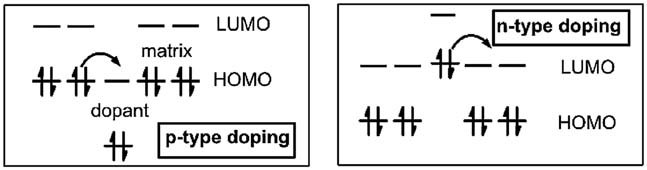
\includegraphics[width=12cm]{Images/doping.jpg}
  \caption{Schemes for p-type (left) and n-type (right) doping processes. Extracted from reference \cite{lussemDopingOrganicSemiconductors2013}.}
  \label{fig:doping}
\end{figure}

The use of small molecules is commonly reported as dopants for organic materials. Some strong acceptor (or electron-defficient) molecules that are widely used are 2,3,5,6 tetrafluoro-7,7,8,8-tetracyanoquinodimethane (F$_{4}$TCNQ) or 1,3,4,5,7,8 hexafluoro-7,7,8,8-tetracyanonaphthoquinodimethane (F$_{6}$TCNQ), which also take part in this work. The latter exhibits a higher electronic affinity (-5.3 eV) or deep HOMO than F$_{4}$TCNQ (-5.2eV) meaning that it can abstract more electrons, specially to polymers with low ionization potential (less than 5eV) or shallow LUMO, \cite{kieferDoubleDopingConjugated2019}, as it is the case of p(g3T2-T) acting as donor.

\begin{figure}
  \centering
  \includegraphics[width=10cm]{Images/dopingprocess.png}
  \caption{Energy diagram of p(g3T2-T) with a) F$_{6}$TCNNQ and b) F$_{4}$TCNNQ. Ionization potential of p(g3T2-T) extracted from reference \cite{tanTuningOrganicElectrochemical2022} and electron affinities of the neutral species (EA$^{0}$) and of the anion (EA$^{-}$) of the dopants are extracted from reference \cite{kieferDoubleDopingConjugated2019}.}
  \label{fig:doping}
\end{figure}

Among the different methods to molecular doped a material, Jacobs et al. compared a solution-mixed and solution sequential doping of P3HT:F4TCNQ films, both straighforward and easy methods to dope thin films \cite{jacobsComparisonSolutionmixedSequentially2016}. In this work it was demonstrated that solution-mixed films are considerably rougher than solution-sequential films, affecting negatively to its conductivity. The fact that solution-sequential doped films allows better homogeneity, make it also more compatible with microstructuring processes such as photolithography. At the expense of enabling easier and more precise control of doping levels \cite{tanOrganicMixedIonic2022}.


%\subsubsection{Techniques for doping conjugated polymers}

%\subsubsection{Measuring techniques to characterize doping}

\section{Organic Mixed Ionic/Electronic Conductors (OMIECs)}

Organic Mixed Ionic/Electronic conductors are organic semiconductors that allow the conduction of electrons (or holes) and ions, the latter set them apart from other organic semiconductors. %Electronic charges accumulated on the conjugated polymer backbone result in secondary property changes in electrochemical potential and electronic conductivity \cite{tanOrganicMixedIonic2022}. 
Initially investigated for batteries and super capacitors, %copy references from paper of Paulson?
where the induction of charges in a semiconducting polymer was the main objective, OMIECs has rapidly grown to include other applications, among them, our focus: OECTs.\\
Paulsen et al. classified OMIECs into six different categories according to their phase and ionic link \cite{paulsenOrganicMixedIonic2020}, details are shown in Figure \ref{fig:omiectypes}. 


% PEDOT:PSS Heterogeneous, blends or complexed systems OMIEC. Conjugated polymer/electrolyte blends. Contains ions chemically linked ot an insulating or conjugated component
% p(g3T2-T) Homogeneous, single-component systems OMIEC. Conjugated polymer electrolytes. Ions introduced as free species upon material casting or device operation

\begin{figure}
  \centering
  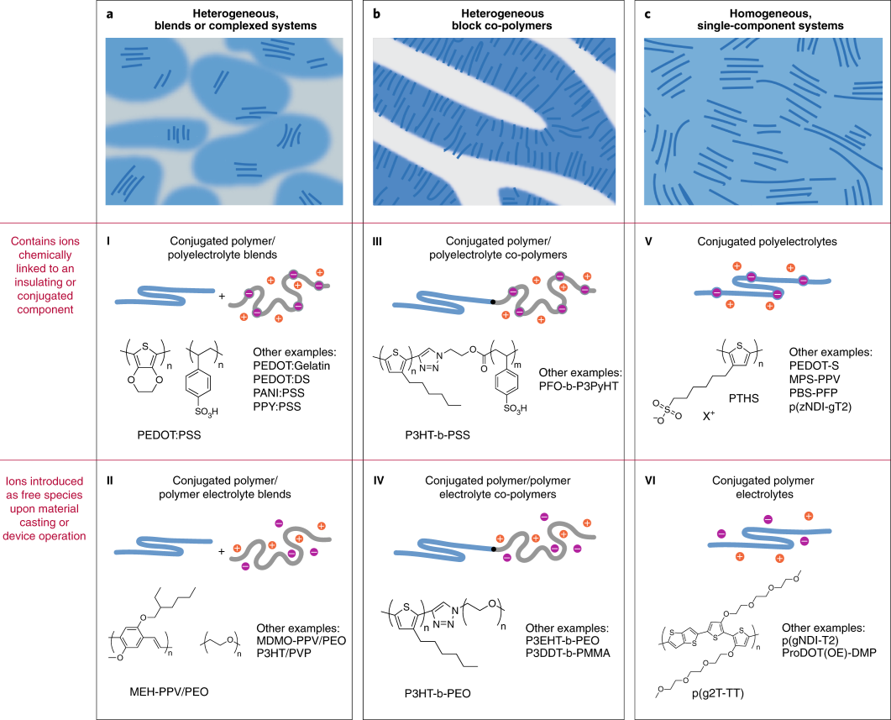
\includegraphics[width=\textwidth]{Images/OMIEC_types.png}
  \caption{\textbf{Material classes of OMIECs.} a) Heterogeneous blends of an electronically conducting conjugated polymer with (I) an ionic charge bearing polyelectrolyte or (II) an ion solvating polymer electrolyte. %These systems frequently feature impure phases and can be largely disordered on multiple length scales. 
  b) Heterogeneous block copolymers of an electronically conducting conjugated polymer with (III) an ionic charge bearing polyelectrolyte or (IV) an ion solvating polymer electrolyte. %Such block copolymers often feature more well-defined pure phases and mesoscale order—readily synthetically tunable. 
  c) Fully conjugated (V) ionic charge bearing polyelectrolytes and (VI) ion solvating polymer electrolytes. %OMIEC types I–IV produce heterogeneous morphologies with microphase segregated predominately electron conducting and ion conducting domains. As shown in the sketches in the first row, in the case of blends (I and II) this occurs in a disordered fashion, or in the case of block copolymers (III and IV) it can occur in a variety of ordered structures (lamellar phase portrayed here). All-conjugated polyelectrolytes (V) and polymer electrolytes (VI) exist as a single mixed conducting phase that may contain heterogeneous composition of ordered and amorphous domains. Conceptual sketches (grey, ionic transport component; blue, electronic transport component; orange, cations; magenta, anions) 
  Extracted from reference \cite{paulsenOrganicMixedIonic2020}.}
  \label{fig:omiectypes}
\end{figure}




\subsection{A widely used material: PEDOT:PSS}
%\subsection{Engineering of semiconducting polymers}
Poly(3,4-ethylenedioxythiophene) poly(styrene-sulfonate) (PEDOT:PSS) is an organic conducting polymer that is widely used in multiple applications in organic electronics. Classified as type I OMIEC according to Paulsen et al, it is a blend between a conjugated polymer (PEDOT) and a polyelectrolyte (PSS), the latter posses chemically linked ions.



\subsection{Other Thiophene-based polymers}
%Seria chevere tener un grafico de como thiophene publications empezaron a crecer.
Thiophene is a planar conjugated ring structure consists of six delocalized pi-electrons. The aromatic nature arises from the four pi electrons and one unshared lone pair of electrons of the oxygen as six delocalized pi-electrons. It folow Hucke´s rule. Hene it is aromatic compound



Organic semiconductors with polar sidechains have been identified as a promising class of materials for the field of bioelectronics. These materials, also called organic mixed ionic/electronic conductors (OMIECs), can exchange ions with aqueous electrolytes when electronic charge carriers are injected, transported, and stored in the bulk of the material \cite{giovannittiEnergeticControlRedoxActive2020}

%Homogeneous single phase OMIECs (types V and VI) display larger magnitudes of ionic–electronic coupling and larger values of volumetric capacitance than biphasic OMIECs (types I–IV) \cite{paulsenOrganicMixedIonic2020}. 

Under the classification shown in Figure \ref{fig:omiectypes}, p(g3T2-T) can be identified as a type VI OMIEC that comprises a conjugated polymer with ions introduced as \textbf{free species} wheareas PEDOT:PSS' ions are \textbf{chemically linked} to the polyelectrode (PSS) and blended to the conjugated polymer (PEDOT). This structural characteristic make p(g3T2-T) display larger magnitudes of ionic-electronic coupling but at the same time will be important for understanding the challenges on having a stable OECT with our material and will be bring back in Section \ref{subsec:req}.

%actually from reference 44, benchmarking omiecs for transistors

\subsection{Electrochemical Doping}

The electrochemical charging of OMIECs can be described as a capacitive faradaic charging process,
% there is current caused by charge transfer, other physical phenomenas such as desorption or adsorption can also lead to the aparition of current that is non faradaic reaction
meaning that the OMIEC undergoes a change in its oxidation state (p-doping in the language of physicists) through an electron transfer with the contact (current collector), while ions from the electrolyte penetrate inside the channel material to compensate the carge carrier on the polymer backbone electrostatically with no change in the inserted ion's oxidation state \cite{giovannittiEnergeticControlRedoxActive2020}  

Savva et al. study the influence of water on the performance of OECT, the water uptake of conjugated polymer films led to 10-13\% mass increase under non biased conditions. As the concentration of water decrease (NaCl$_{aq}$ 10 mM, 100mM, 1M, and 6M) ionic charging is faster regardless of the doping pulse, however the fastest ionic charging is achieved at NaCl$_{aq}$ 1 M. The injection/drift of ions is also affected by the ion-counterion attractive forces which delays the ion injection from the electrolyte, opposing their drift into the polymer (NaCl$_{aq}$ 6 M hinders the drift of anions) affecting the response time. \cite{savvaInfluenceWaterPerformance2019}

\section{Organic Electrochemical Transistors (OECTs)}

Organic Electrochemical Transistors (OECTs) consists of metallic source, drain and gate electrodes, an organic semiconductor channel (specifically an OMIEC as described in previous section) and an electrolyte that couples channel and gate \cite{rivnayOrganicElectrochemicalTransistors2018}

\begin{figure}[ht]
	\centering
	\subfloat[]{{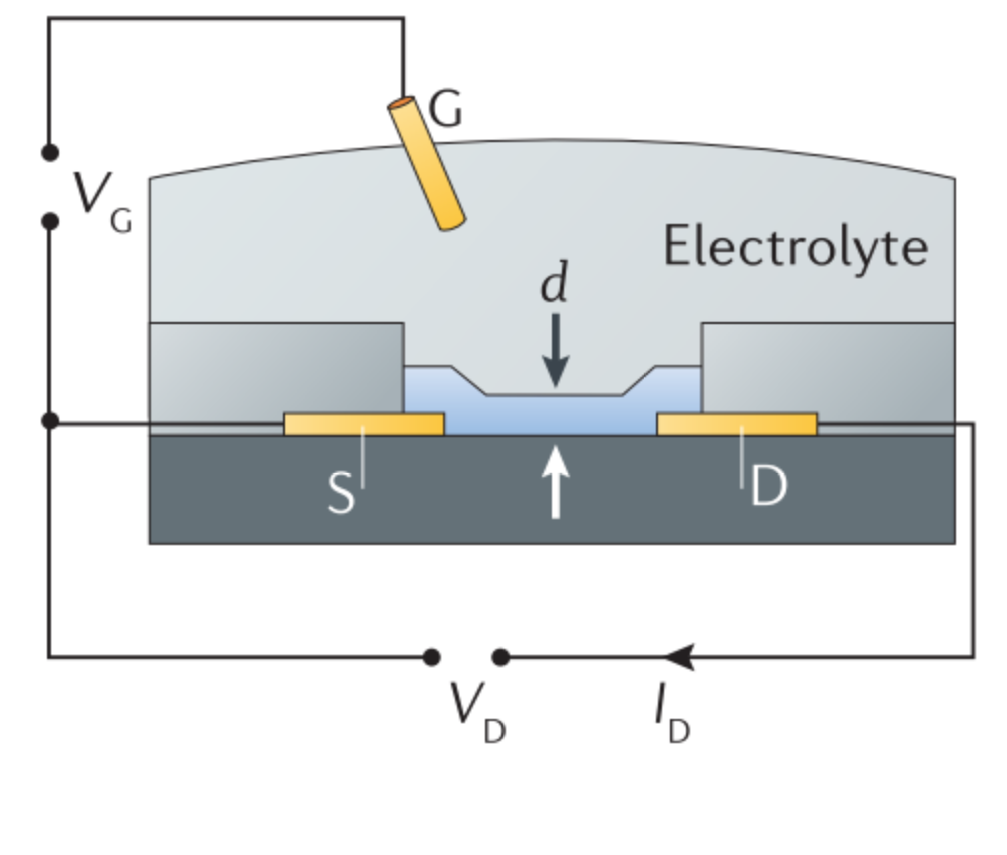
\includegraphics[height=4.5cm]{Images/structure.png} }}
	\qquad
	\subfloat[]{{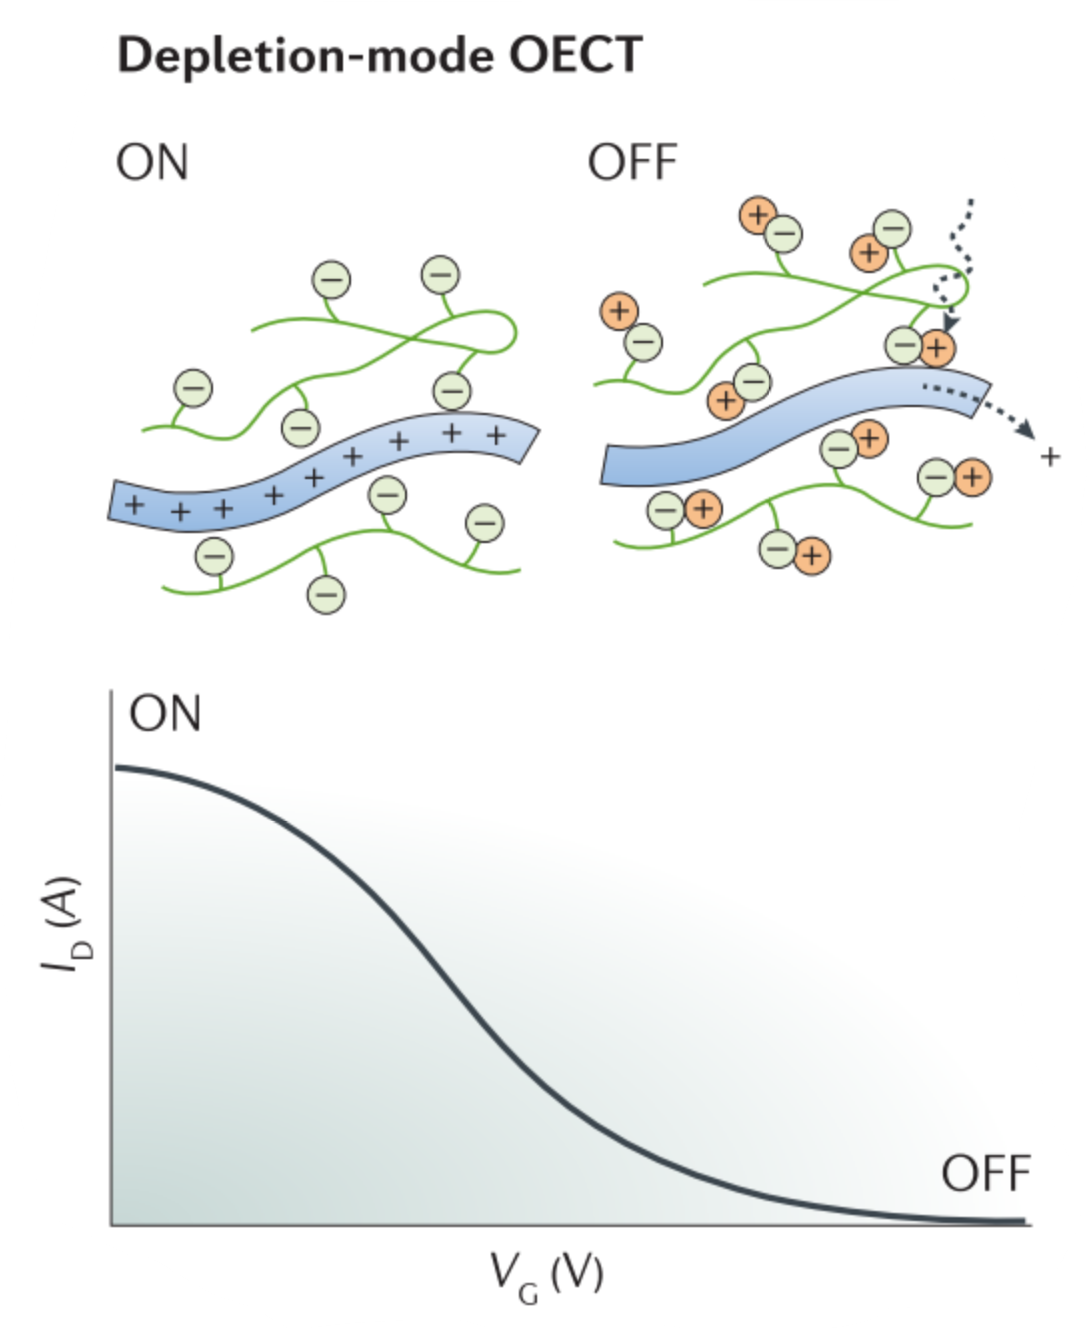
\includegraphics[height=8cm]{Images/depletion.png} }}
	\subfloat[]{{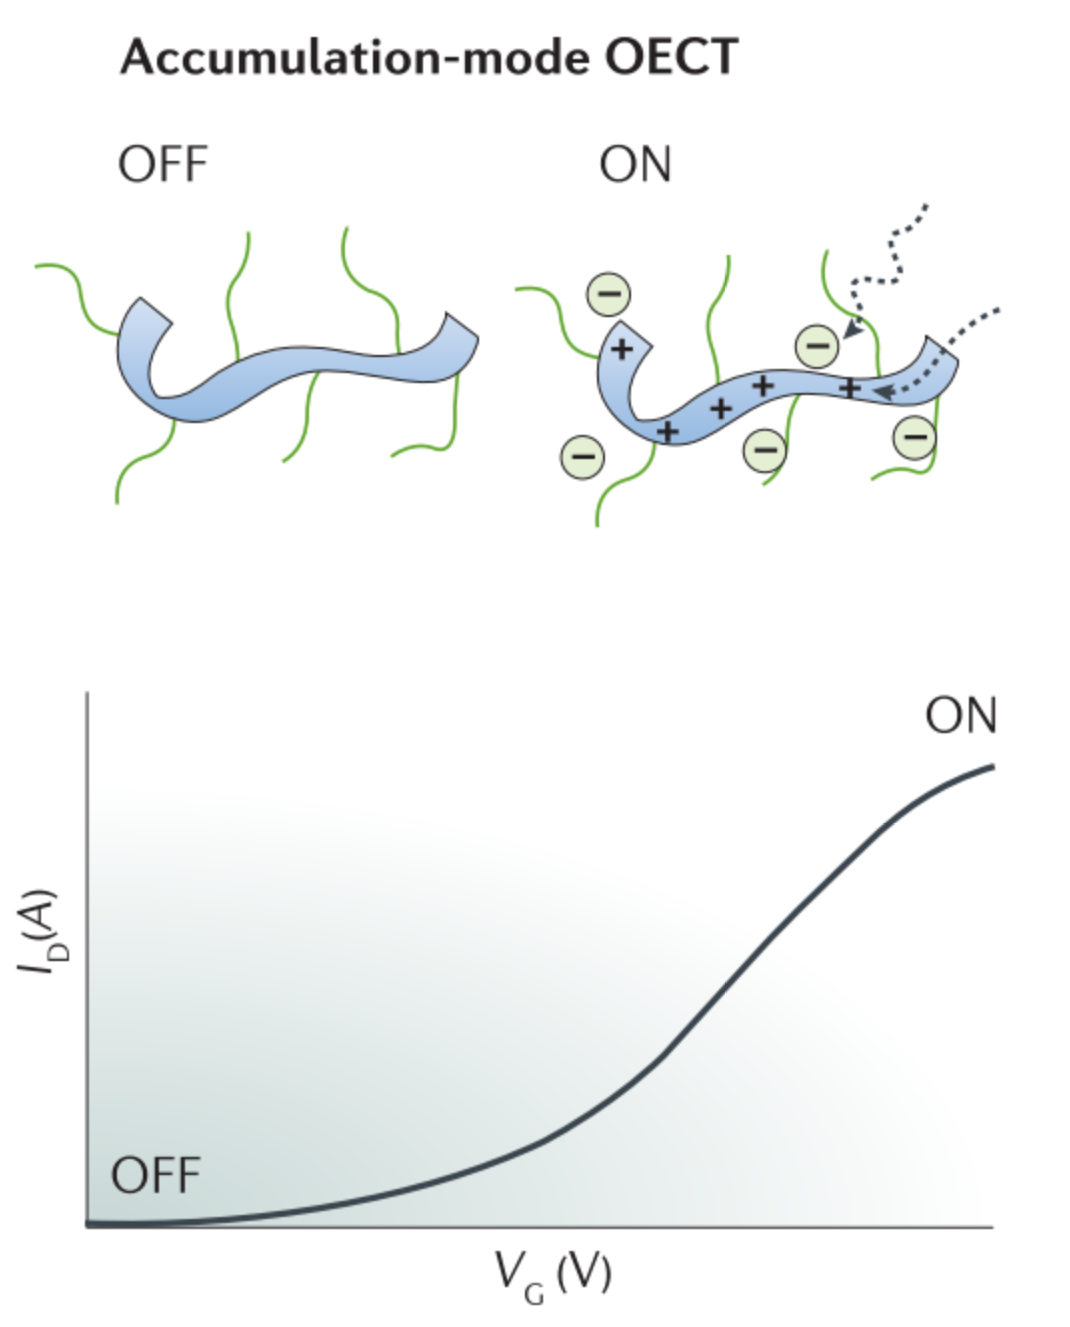
\includegraphics[height=8cm]{Images/accumulation.png} }}
	\caption{(a) Typical structure of an organic electrochemical transistor (OECT). (b) Transfer curve showing depletion-mode operation of an OECT with a conducting polymer channel. (c) Transfer curve showing accumulation-mode operation of an OECT with a semiconducting polymer channel. Images extracted from reference \cite{rivnayOrganicElectrochemicalTransistors2018}.}
	\label{fig:modes}
\end{figure}

The semiconductor

%devices that are mechanically compliant, biocompatible, and are sensitive to biochemical modules \cite{tanMixedIonicElectronic2022} 

\subsection{Device Physics}

\subsection{Operation Modes}

Due to its commercial availability, operational stability, and relatively high performance, PEDOT:PSS became a standard material for p-type OECTs. Its main drawback lays in its depletion-mode operation, which requires a voltage to turn off the device (as represented in Figure 1(b)). With the aim of minimizing power consumption, there is a special interest to design semiconducting polymers that would allow accumulation-mode devices (Figure 1(c)) with high performance \cite{nielsenMolecularDesignSemiconducting2016} \cite{tanOrganicMixedIonic2022}.

Accumulation-mode devices has the advantage of dissipating less static power when the device is not operated, due to low OFF current, which must be minimized as much as possible \cite{giovannittiEnergeticControlRedoxActive2020}

Nielsen et al. reported a series of semiconducting polymers with Ethylene Glycol (EG) side chains designed to elucidate important strcuture-property guidelines for accumulation-mode OECT operation. They demonstrated that an OECT with 3-(2-(2-(2-methoxyethoxy)ethoxy)ethoxy)thiophene p(g3T2-T), as seen in Figure , has higher transconductance, and a turn-on voltage close to zero compared to other thiophene-based species \cite{nielsenMolecularDesignSemiconducting2016}. While its backbone design warrant reversibility during electrochemical redox reactions and good electronic transport, the EG side chains enable its stability in aqueous electrolytes and efficient transport of ionic and electronic charge carrier \cite{moiaDesignEvaluationConjugated2019}. Moser et al. studied the impact of the length of the EG side chain of this polythiophene backbone on the performance of OECTs. They reported that reducing chain length would maximize the capacitance, but the increase of length would enhance ion-polymer interaction. Finally, they suggested an optimum length of 3 monomers in side chains over 2, 4 and 6 monomers \cite{moserEthyleneGlycolBasedSide2020}. The main advantage of p(g3T2-T) over PEDOT:PSS is its higher transconductance \cite{nielsenMolecularDesignSemiconducting2016}, the absence of extensive pre- and postprocessing to optimize polymer stability and electrochemical performance in aqueous media and the possibility of an accumulation-mode OECT with low operation voltages\cite{moserEthyleneGlycolBasedSide2020}.

\subsection{Important Figures of Merit}

\subsubsection{Transconductance}

\subsubsection{$\mu$C* product}

\subsubsection{Threshold voltage}

An approach to shift the operating voltage range for PEDOT:PSS OECTs to lower the channel current, leading to reduced power consumption, is to tune the threshold voltage by de-doping PEDOT:PSS using commercially available amine-based molecular de-dopants \cite{keeneEnhancementModePEDOTPSS2020}. Tan et al., on the other hand, explored a different approach, rather than modifying the doping level of the channel, they tuned the doping level of the gate to shift the threshold voltage. They used p(g3T2-T) and obtained a 400mV change with 60\% mol ratio of 2,3,5,6-Tetrafluoro-7,7,8,8-tetracyanoquinodimethane (F4TCNQ) dopant. The advantage over this approach is i) protecting the material from oxidation, since the Fermi level in brought towards the highest occupied molecular orbital (HOMO), and ii) no interference with the channel which helps to leave the transconductance unaffected \cite{tanTuningOrganicElectrochemical2022}.

{\subsection{Requirements to Avoid Undesirable Side Reactions}}
\label{subsec:req}

Achieving effective charge transfer between the analyte and OMIEC requires appropriate alignment of the electrochemical potential of electrons on the OMIEC electrode and the redox specie. Failure to do so may result in the subsequent transfer of charges to other redox-active sinks in the environment, leading to undesirable side reactions and products that may interfere with the OMIEC’s operation. Electrons flow from a region of higher to lower electrochemical potential. Hence, achieving electron transfer from redox-active species to the OMIEC requires the latter to have a deep LUMO (high electron affinity) \cite{tanMixedIonicElectronic2022} %paper

\subsubsection{Oxygen Reduction Reaction (ORR)}

With the aim of developing accumulation-mode OECTs, the engineering of new OMIECs were introduced as commented in previous sections. Normally, this polymer backbones have low ionization potential (IPs) which lead to another side effect issue that little attention has been paid: non capacitive faradaic rections in ambient: electron-transfer reaction from the OMIEC to molecular oxygen described as oxygen reduction reaction (ORR)

% Remember 
% Thermodynamically favored processes or reactions are those that involve both a decrease in the internal energy of the components (ΔH° < 0) and an increase in entropy of the components (ΔS° > 0). These processes are necessarily “thermodynamically favored” (ΔG° < 0) or negative. ΔG° = ΔH°-TΔS°
% Catalyst help to reduce the activation energy required for a reaction

The ORR yields either H$_{2}$O$_{2}$ or water (H$_{2}$O) as well as charging (oxidation) of the OMIEC that acts as the catalyst. The first shows a free energy difference that is endergonic for OMIECs with IPs \> 4.9eV and hence prevent the OMIEC from undergoing ORR that form H$_{2}$O$_{2}$. To prevent the ORR in ambient conditions, OMIECs based on donor-acceptor copolymer (Type III or IV) that have large IPs to shift
\cite{giovannittiEnergeticControlRedoxActive2020}
% Actually this material does not avoid this, we need to take into account this interaction.

\subsection{Building Block for neuromorphic and bioelectronic applications}



%%% Local Variables: 
%%% mode: latex
%%% TeX-master: "thesis"
%%% End: 
